\section{Learning Agents}
A learning agent is an agent who can operate in unfamiliar environments and can improve its knowledge by learning from experiences.

\begin{figure}[ht]
    \centering
    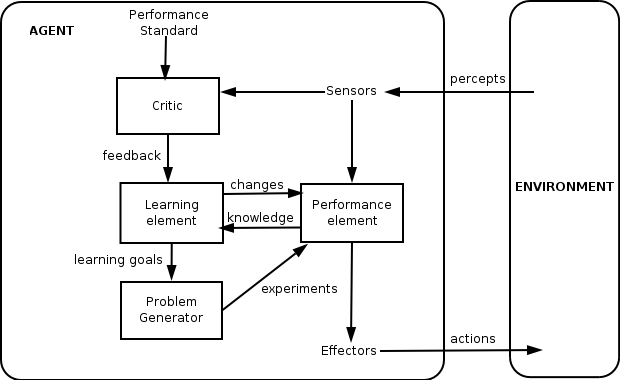
\includegraphics[width=0.4\textwidth]{images/IntelligentAgent-Learning.png}
    \caption{Learning agent.}
\end{figure}

\noindent
A learning agent can be divided into four conceptual elements:
\begin{itemize}
    \item \textbf{Performance element}: Perceives the environment and performs actions.
    \item \textbf{Critic}: Tells the learning element how well the agent is doing with respect to a fixed performance standard \cite{russell2002artificial}.
    \item \textbf{Learning element}: Improves the performance element given the feedback from the critic.
    \item \textbf{Problem Generator}: Suggests actions to the agent to explore new experiences.
\end{itemize}
The performance standard is needed to help establish the quality of agent behavior.

\vspace*{4mm}
\noindent
Agent behavior is described by a policy $\pi$ which decides what action to take in a given state.
To evaluate whether the policy is good or not, a utility function $U^{\pi}$ is used.
The policy with the largest utility value is called optimal policy.
There are several ways to improve the policy and to make the agent learn.
